% Parameter Sensitivity Analysis (Fig. 7) - Vertical Single-Column Layout (2x1)
% Compile: pdflatex fig_sens_A2.tex -> fig_sens_A2.pdf
\documentclass[border={4pt 18pt 4pt 4pt}]{standalone}
\usepackage{tikz}
\usepackage{pgfplots}
\pgfplotsset{compat=1.18}
\usepgfplotslibrary{fillbetween}

\definecolor{daliablue}{RGB}{0, 0, 235}
\definecolor{wesadcyan}{RGB}{0, 165, 230}

\begin{document}
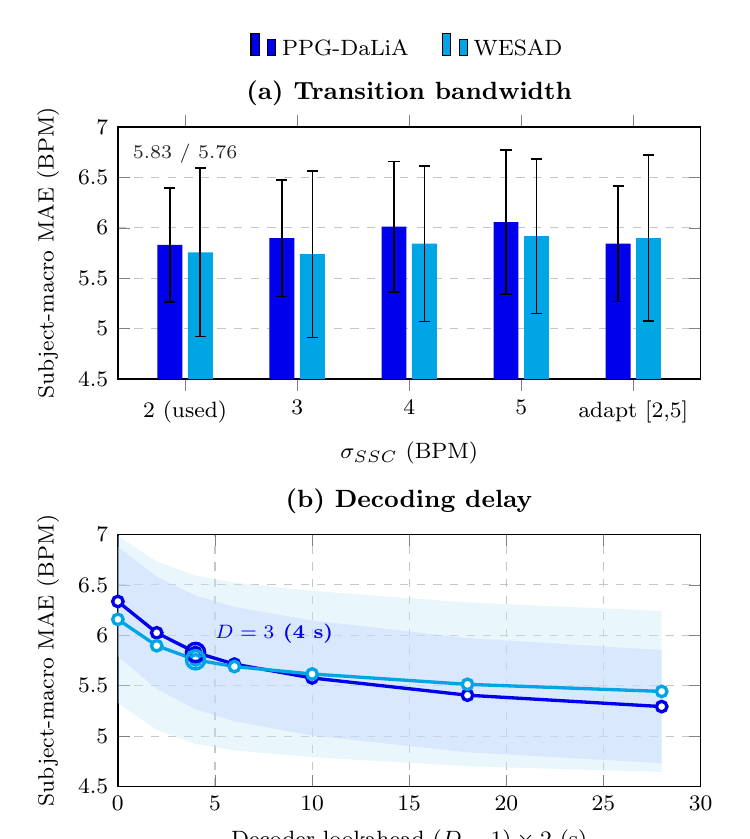
\begin{tikzpicture}

% ---- Top Panel: (a) Transition bandwidth sigma_SSC ----
\begin{axis}[
    name=ax1,
    width=7.4cm,
    height=3.2cm,
    scale only axis,
    ybar=2pt,
    bar width=9pt,
    ymin=4.5, ymax=7.0,
    xmin=0.4, xmax=5.6,
    xtick={1, 2, 3, 4, 5},
    xticklabels={2 (used), 3, 4, 5, {adapt [2,5]}},
    ytick={4.5, 5.0, 5.5, 6.0, 6.5, 7.0},
    xlabel={$\sigma_{SSC}$ (BPM)},
    ylabel={Subject-macro MAE (BPM)},
    title={\textbf{(a) Transition bandwidth}},
    title style={yshift=-2pt, font=\small},
    ymajorgrids=true,
    grid style={dashed, gray!45, line width=0.4pt},
    legend style={at={(0.5,1.22)}, anchor=south, legend columns=2, font=\footnotesize, draw=none, fill=none, /tikz/every even column/.append style={column sep=10pt}},
    tick label style={font=\footnotesize},
    label style={font=\footnotesize},
    axis line style={line width=0.6pt}
]

\addplot[
    fill=daliablue, draw=none,
    error bars/.cd, y dir=both, y explicit,
    error bar style={black, line width=0.6pt},
    error mark options={rotate=90, black, mark size=2pt, line width=0.6pt}
] coordinates {
    (1, 5.8302) +- (0, 0.5641)
    (2, 5.8979) +- (0, 0.5786)
    (3, 6.0114) +- (0, 0.6484)
    (4, 6.0580) +- (0, 0.7149)
    (5, 5.8437) +- (0, 0.5745)
};
\addlegendentry{PPG-DaLiA}

\addplot[
    fill=wesadcyan, draw=none,
    error bars/.cd, y dir=both, y explicit,
    error bar style={black, line width=0.6pt},
    error mark options={rotate=90, black, mark size=2pt, line width=0.6pt}
] coordinates {
    (1, 5.7569) +- (0, 0.8354)
    (2, 5.7395) +- (0, 0.8275)
    (3, 5.8435) +- (0, 0.7730)
    (4, 5.9171) +- (0, 0.7681)
    (5, 5.8978) +- (0, 0.8223)
};
\addlegendentry{WESAD}

\node[font=\scriptsize, text=black!85] at (axis cs:1, 6.74) {5.83 / 5.76};

\end{axis}

% ---- Bottom Panel: (b) Decoding delay D ----
\begin{axis}[
    name=ax2,
    at={(ax1.below south west)}, anchor=north west, yshift=-0.78cm,
    width=7.4cm,
    height=3.2cm,
    scale only axis,
    xmin=0, xmax=30,
    ymin=4.5, ymax=7.0,
    xtick={0, 5, 10, 15, 20, 25, 30},
    ytick={4.5, 5.0, 5.5, 6.0, 6.5, 7.0},
    xlabel={Decoder lookahead $(D-1)\times 2$ (s)},
    ylabel={Subject-macro MAE (BPM)},
    title={\textbf{(b) Decoding delay}},
    title style={yshift=-2pt, font=\small},
    grid=major,
    grid style={dashed, gray!45, line width=0.4pt},
    tick label style={font=\footnotesize},
    label style={font=\footnotesize},
    axis line style={line width=0.6pt}
]

% Shaded SEM bands
\addplot[name path=dalia_hi, draw=none, forget plot] coordinates {
    (0, 6.8800) (2, 6.5822) (4, 6.3943) (6, 6.2821) (10, 6.1480) (18, 5.9725) (28, 5.8542)
};
\addplot[name path=dalia_lo, draw=none, forget plot] coordinates {
    (0, 5.7916) (2, 5.4680) (4, 5.2661) (6, 5.1461) (10, 5.0056) (18, 4.8395) (28, 4.7320)
};
\addplot[daliablue!22, fill opacity=0.45, forget plot] fill between[of=dalia_hi and dalia_lo];

\addplot[name path=wesad_hi, draw=none, forget plot] coordinates {
    (0, 6.9883) (2, 6.7318) (4, 6.5923) (6, 6.5237) (10, 6.4418) (18, 6.3265) (28, 6.2425)
};
\addplot[name path=wesad_lo, draw=none, forget plot] coordinates {
    (0, 5.3281) (2, 5.0620) (4, 4.9215) (6, 4.8569) (10, 4.7906) (18, 4.7011) (28, 4.6443)
};
\addplot[wesadcyan!22, fill opacity=0.40, forget plot] fill between[of=wesad_hi and wesad_lo];

% Mean curves
\addplot[color=daliablue, line width=1.2pt, mark=*, mark size=1.9pt, mark options={fill=white, solid}] coordinates {
    (0, 6.3358) (2, 6.0251) (4, 5.8302) (6, 5.7141) (10, 5.5768) (18, 5.4060) (28, 5.2931)
};
\addplot[color=wesadcyan, line width=1.2pt, mark=*, mark size=1.9pt, mark options={fill=white, solid}] coordinates {
    (0, 6.1582) (2, 5.8969) (4, 5.7569) (6, 5.6903) (10, 5.6162) (18, 5.5138) (28, 5.4434)
};

% Highlight operating point D = 3 (4 s lookahead)
\addplot[only marks, color=daliablue, mark=o, mark size=3.3pt, line width=1.2pt, forget plot] coordinates {(4, 5.8302)};
\addplot[only marks, color=wesadcyan, mark=o, mark size=3.3pt, line width=1.2pt, forget plot] coordinates {(4, 5.7569)};
\node[font=\scriptsize\bfseries, text=daliablue, anchor=south west] at (axis cs:4.5, 5.82) {$D = 3$ (4~s)};

\end{axis}

\path (ax2.below south) +(0,-4pt);

\end{tikzpicture}
\end{document}
